\chapter{LOCAL MOTOR INVARIANT}
\label{chap:li}

\nomenclature[f1]{$G$}{A Lie Group}
\nomenclature[f2]{$g_a$}{an element in Lie Group $G$ with parameter $a$}
\nomenclature[f3]{$\iv(x)$}{Invariant Function of $x$}
\graphicspath{{LocalInvariant/LocalInvariantFigs/EPS/}{LocalInvariant/LocalInvariantFigs/}}


\section{Qunatative Properties of Motion}
Global Motor Invariant Control maintains motion stablity.
To make motions realistic, some natural looking features should also be preserved.
Some features of motions such as smoothness or energy efficient are quantative.
\cms research should provide a framework perserving feature.
Another question missiong is animals can finish motion tasks require high accuracy.

These are the motivations for the development of \emph{Local Motor Invariant}.
Local Motor Invariants are quantative properties of motions, the idea of invariant perserving are abstracted as the ``Symmery'' and Group theory.
Features are modelled as symmetrical functions, while feature preserving actions form a group.
From dynamic perspective, motions are solutions to dynamic equations.
The actions transform one motion to another close related to the Lie Group Theory for differential equations\citep{olver1986applications}.

The introduction of Lie Group not only provides a powerful mathematical tools for modelling the symmetry property, but also provides an idea to simplify the solving the dynamics.

\subsection{Group and Symmetry}
For the more traditional geometrical perspective, ''Symmetry''  means a geometry is the same after transformation.
For the example of a square,  $90$ degree clockwise rotation will make it the same, as shown in Figure~\ref{fig:symsquare}.
\begin{figure}[!htbp]
  	\begin{center}
   	\includegraphics[width=0.7\textwidth]{Symmetry}
	\end{center}
	\caption{Symmetry of The Square}
    \label{fig:symsquare}
\end{figure}

The actions that preserve the shape have some properties.
For example, if the $90$ degree clockwise rotation preserve the shape, then rotate twice will also preserve the symmetry, that's equal to asy $180$ degree clockwise roatation also preserve the symmetry.

All the action that can preserve the symmetry form a group $G$.
A group has the following properties.
\begin{enumerate}
\item For any $g_a,g_b$ in $G$, \,$g_a*g_b$\, belongs to $G$. (The operation
``$*$'' is closed).

\item For any \,$g_a,g_b,g_c\in G$, \,$(g_a*g_b)*g_c=g_a*(g_b*g_c)$. \,(Associativity of
the operation).

\item There is an element $e\in G$ such that \,$g_a*e=e*g_a=g_a$\, for any
\,$g_a\in G$. (Existence of identity element).

\item For any \,$g_a\in G$\, there exists an element $g_h$ such that
\,$g_a*g_h=g_h*g_a=e$. \,(Existence of inverses).
\end{enumerate}

For the square example, $g_1$ is  $90$ degree clockwise rotation. then $e$ is no rotation.
$g_2=g_1*g_1$ is rotate $90$ degree clockwise twice.$g_2$ is a element of the group $G$, then $g_2$ preserve symmetry.


From algebra perspective, ``Symmetry'' means the value of function is invariant after varaible transformation.
For a function $\iv (x)$,
The group transformation is define by $\hat{x}=g_a(x)$
By symmetry, we mean $\iv (x)=\iv (\hat{x})$.
$\iv(x)$ is an invariant function of group $G$.

Note that  the shape invariant by actions in $G$ is not unique.
Many shapes are invariant, and the combination of two invariant shapes also form an invariant shape. 
The invariant shapes form a space, the invariant space $\iv (x)$.


\begin{figure}[!htbp]
  \begin{center}
    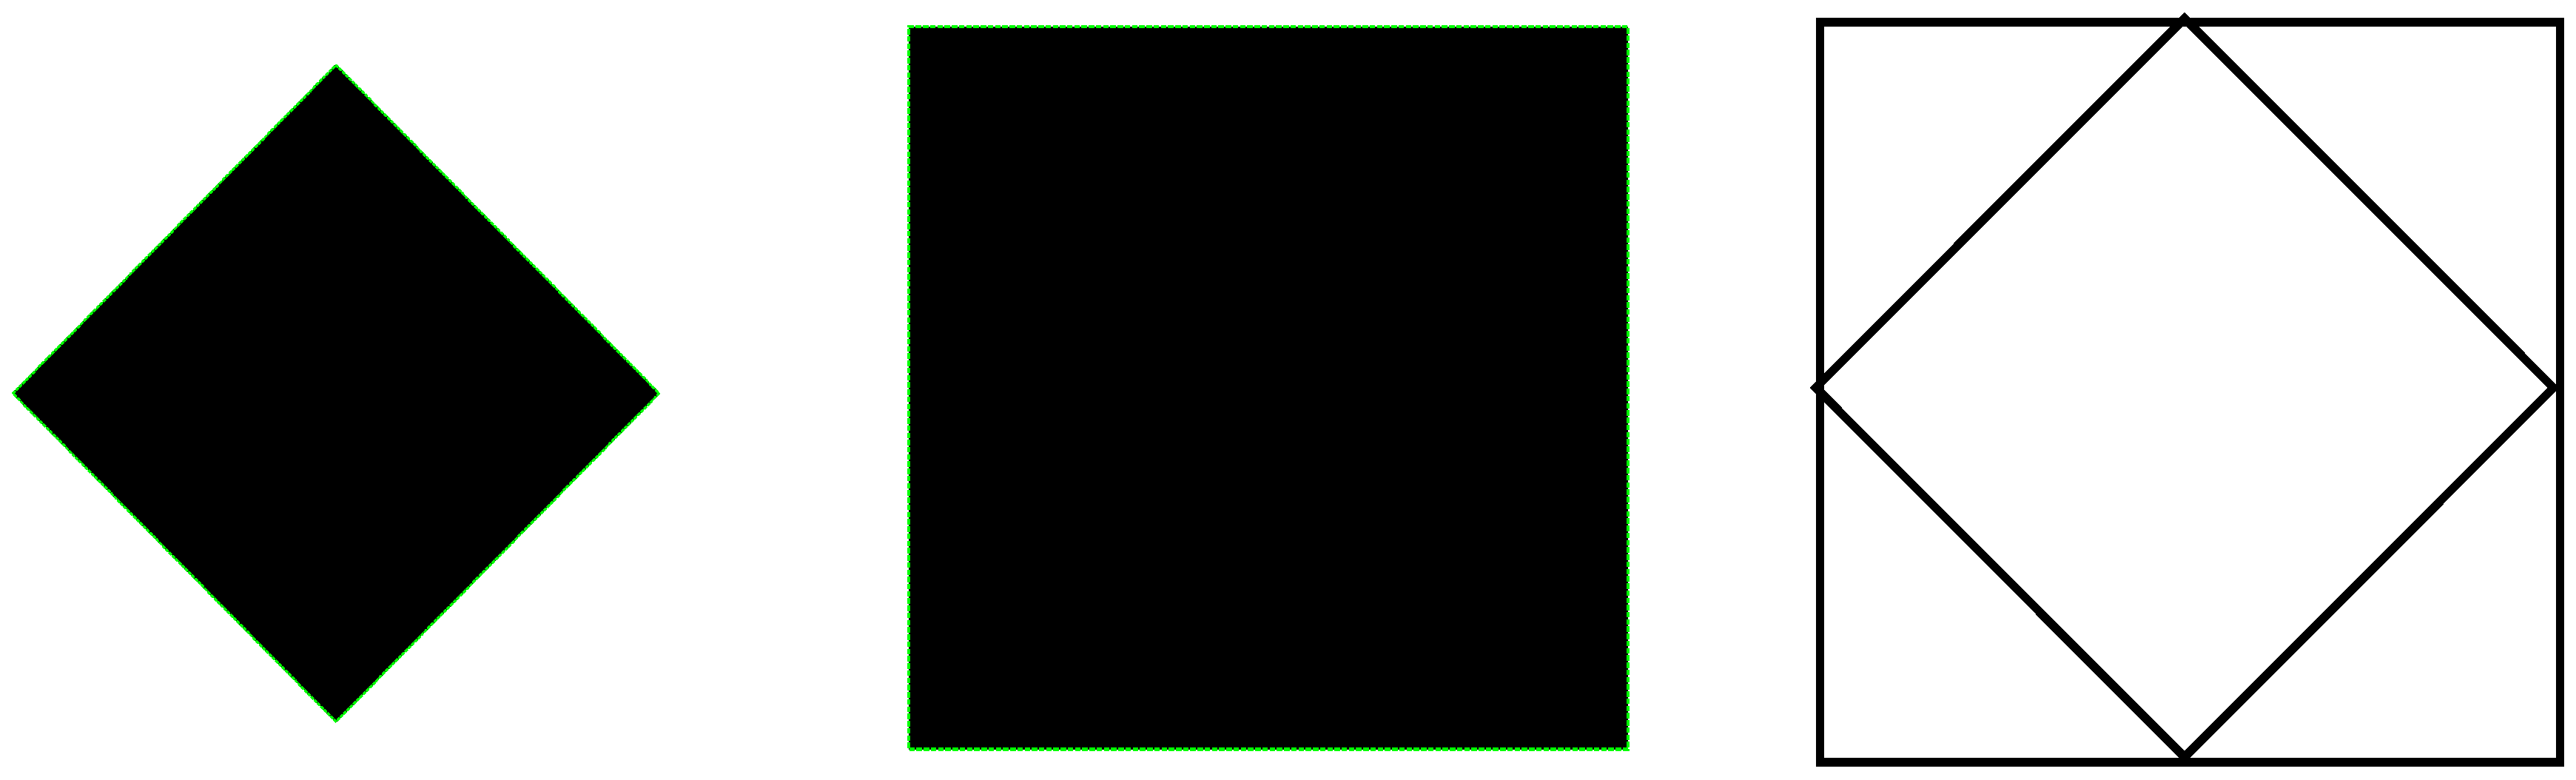
\includegraphics[width=0.7\textwidth]{SymmetrySpace}
    \caption{Symmetry Space}
    \label{fig:symmetry Space}
\end{center}
\end{figure}





\subsection{Lie Group and Symmetry of Dynamic System}
The rotate group is discrete.
For the circle, the rotation is continuous.
The continuous group is a Lie Group.

Lie Group originates from study of differential equation.
For Physically-based animation,
Motion is usually described by
\begin{equation}
	\dot{\state}=F(\state)
\end{equation}
Lie Group $G$ will preserve the differential equation, for $g_a \in G$ 
\[
Tg_a(\dot{\hat{\state}})=F(g_a(\state)
\]
where $Tg_a$ is the corresponding lift action that transform the velocity $\dot{\state}$.

for example, if the $g_a$ is translate transformation, velocity will not be translate, then $Tg_a$ is identity.





Physically possible motion is the solution of the equation.
An important property from one solution $\state(t)$.
with a group action $g_a$, we can get another solution $g_a(\state(t))$
 	
for the mass spring system ~\ref{eq:stateform}
we apply the group action 
\[
\hat{\state}=g_a(\state)=[\alpha q, \alpha \qd ]
\]
then the lift action is
\[
\dot{\hat{\state}}=Tg_a(\state)=[\alpha \qd, \alpha \ddot{q}]
\]



by substitution $\state \mapsto \hat{\state}$, the original system become
\[ 
\dot{\hat{\state}}=
\left[ 
\begin{array}{cc}
0 &1\\
-1 &0 
\end{array}
\right]\hat{\state}
\]
which is 
\begin{equation}
\label{eq:tranmas} 
\alpha \dot{\state}=
\left[ 
\begin{array}{cc}
0 &1\\
-1 &0 
\end{array}
\right]\alpha \state
\end{equation}

equation ~\ref{eq:tranmas} is equivalent to  ~\ref{eq:stateform}
thus if $\state(t)$ is a solution, we get another solution $\hat{\state}(t)$.

such transformation form a group.
we define 
\[
g_{\alpha}*g_{\beta}(\state)=[\alpha \beta q, \alpha \beta \qd]
\]
which also satisfy the differential equation.

and 
\[
g_{\alpha}^{-1}=g_{\frac{1}{\alpha}}
\]
when $\alpha \in R^+$, the group is continues,
thus it is an example of Lie Group.





This provide us an idea about motion synthesis.
Given an original motion $q(t)$, and the corresponding group $G$, a new motion is generated by transformation.
For every group G, we can find an function $I(x)$ unchanged by the group action G, 

$I(\state)$ are called local motion invariant. 
For mechanical system,  $I(x)$ has important physically meaning. 
$I(\state)$ corresponding to the Conservative Law like energy or angular momentum.


\section{Controlled Symmetry}
For motion synthesis, usually the desired motion is ma
For example for motion stability, we want the current state is within the basin of attraction.
If we want to control the final motion style, we want the state is on the limit cycle.

For motion synthesis, the problem is given the system, let the original system have the desired symmetry.

 and original motion $m$ is known, but the corresponding group action $g_a$ is not satisfied by differential equation.
For such situation, control input $u$  is added, which modify the original equation to allow the designed $G$, this is called Controlled Symmetry.

Most dynamic motion can be modelled as a Lagrange System. 
\[
L=K(\dot(q)-V(q).
\]
And the desired action $G$ must keep the $L$ invariant. 

The original m is defined by the neural langrage equation
\begin{equation}
\frac{d}{dt} \frac{\partial L}{\partial \qd} - \frac{\partial L}{\partial q} = 0
\label{eq:uncontrolled_euler_lagrange}
\end{equation}
The modified system is 
\begin{align}
\frac{d}{dt} \frac{\partial L}{\partial Tg(\qd)} - \frac{\partial L}{\partial g(q)}&=0,\label{eq:liegroup_euler_lagrange}\\
\frac{d}{dt} \frac{\partial L}{\partial \qd} - \frac{\partial L}{\partial q}&=\ulocal. \label{eq:controlled_euler_lagrange}
\end{align}


(5) and (6) are the equivalent equation, by comparing  equation (5) and (6), we can get $u$
Some Specific examples of Symmetry and Control.
In the following discussion, suppose all the group element $g$ are parameterized by the parameter $\alpha$.

\subsection*{ Offset Action}
we move the posture of the system 
\[
q \mapsto q+\alpha
\]
then the offset transformation is
\[
\goff(\state) = [q+\alpha,\qd]
\]


\begin{equation}
\ulocal(q) = \frac{\partial}{\partial q} \left(V(\goff(q)) - V(q)\right).
\end{equation}

if we formulate the controlled mass spring system in the following way~\ref{eq:controlmass}
\begin{equation}
\label{eq:controlmass}
\ddot{q}+q=\ulocal
\end{equation}

for the mass spring system.
\[
\ulocal(q)=\alpha
\]

\begin{figure}[!htbp]
  \begin{center}
      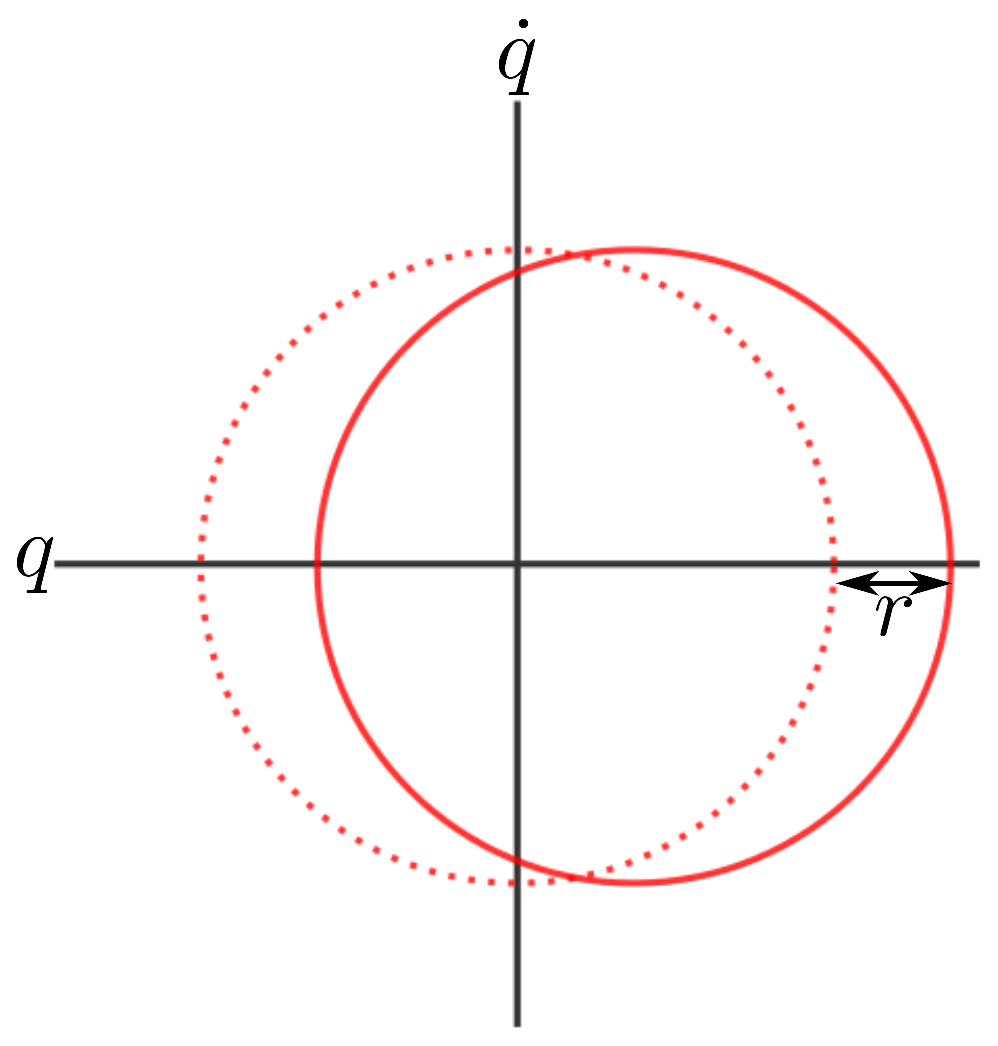
\includegraphics[width=0.7\textwidth]{g_off}
    \caption{Offset Action}
    \label{fig:goff}
\end{center}
\end{figure}
on phase space, if $q$ is the horizontal axis, and $\dot{q}$ is the vertical axis, this has the effect of moving the phase plot horizontally.

\subsection*{Time Scalling}

%g_st(q,dot{q})=(q,st*dot{q})
if we scale the time parameter
\[
t \mapsto \frac{t}{\alpha}
\]

we have
\[
\gts(\state)=[q,\alpha \qd]
\]
\[
T\gts(\dot{\state})=[\alpha \qd,\alpha^2 \ddot{q}]
\]
Then the local control is 
\begin{equation}
\ulocal(q) = (\alpha^2 - 1) \frac{\partial V(q)}{\partial q}.
\end{equation}

for the mass spring system in
\[
\ulocal=(\alpha^2-1)q
\] 

\begin{figure}[!htbp]
  \begin{center}
    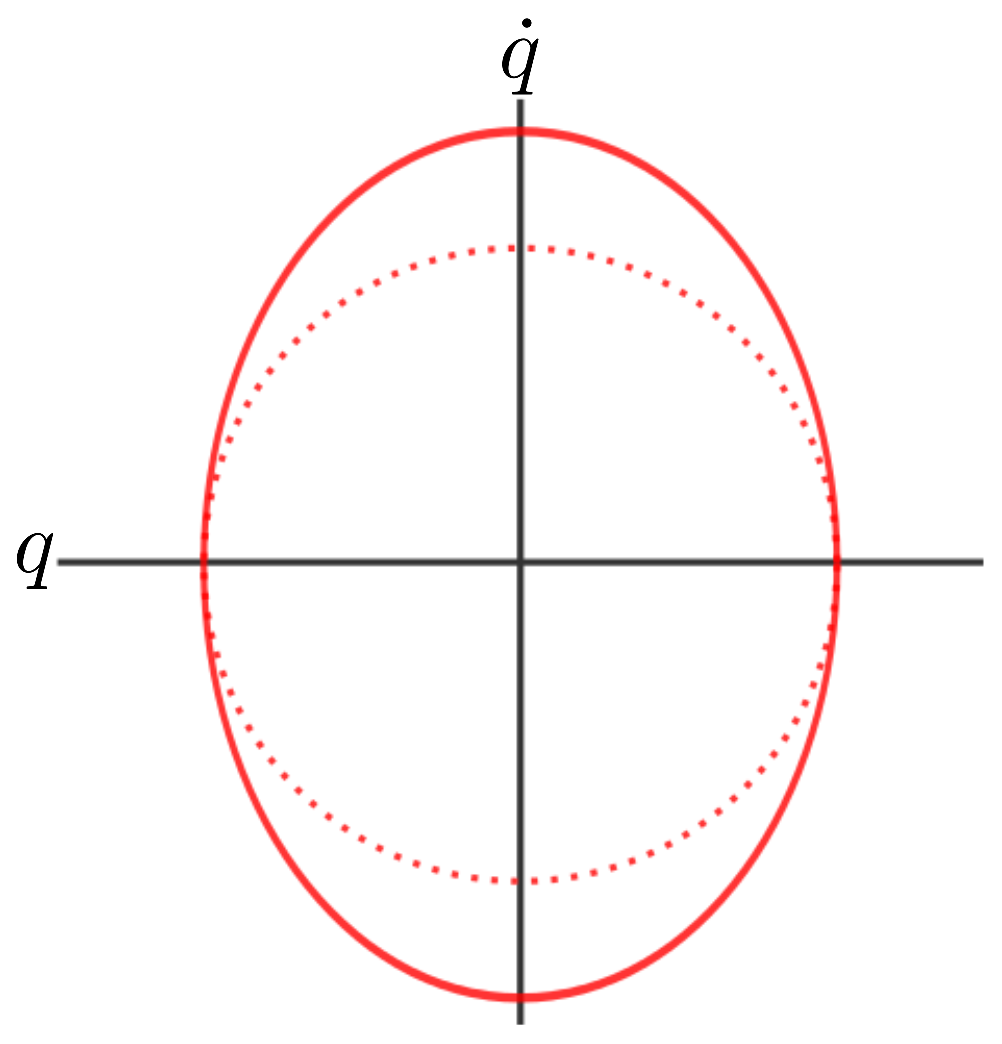
\includegraphics[width=0.7\textwidth]{g_ts}
	 \caption{Time Scaling Action}
    \label{fig:gts}
\end{center}
\end{figure}
on phase space, this has the effect strength the phase plot in the vertical direction

\subsection*{Energy Scaling}
For some system moving the the conservative field.
The energy is preserved and different motion present different level of energy.
For such system, we have the energy $E(\state)=K+V$, where $K$ is the kinematics energy,
$V$ is the potential energy.
\[
E(\hat{\state})=\alpha^2 E(x)
\]
if the mass of system is constant.
\[
\gen(\state)=(f(\alpha) q,\alpha \dot{q}).
\]
where $f(\alpha)$ is a function of $\alpha$, which depends on the shape of potential field.
$\ulocal$ can be developed by applying the pos scaling and time scaling in a combined manner.



for the mass spring system , $E=\frac{1}{2}(q^2+\qd^2)$,$f(\alpha)=\alpha$, and because the energy scaling is kept by the original system, we have
\[
\ulocal=0
\]
On phase plot, this has the effect enlarge the phase portrait.

\begin{figure}[!htbp]
  \begin{center}
      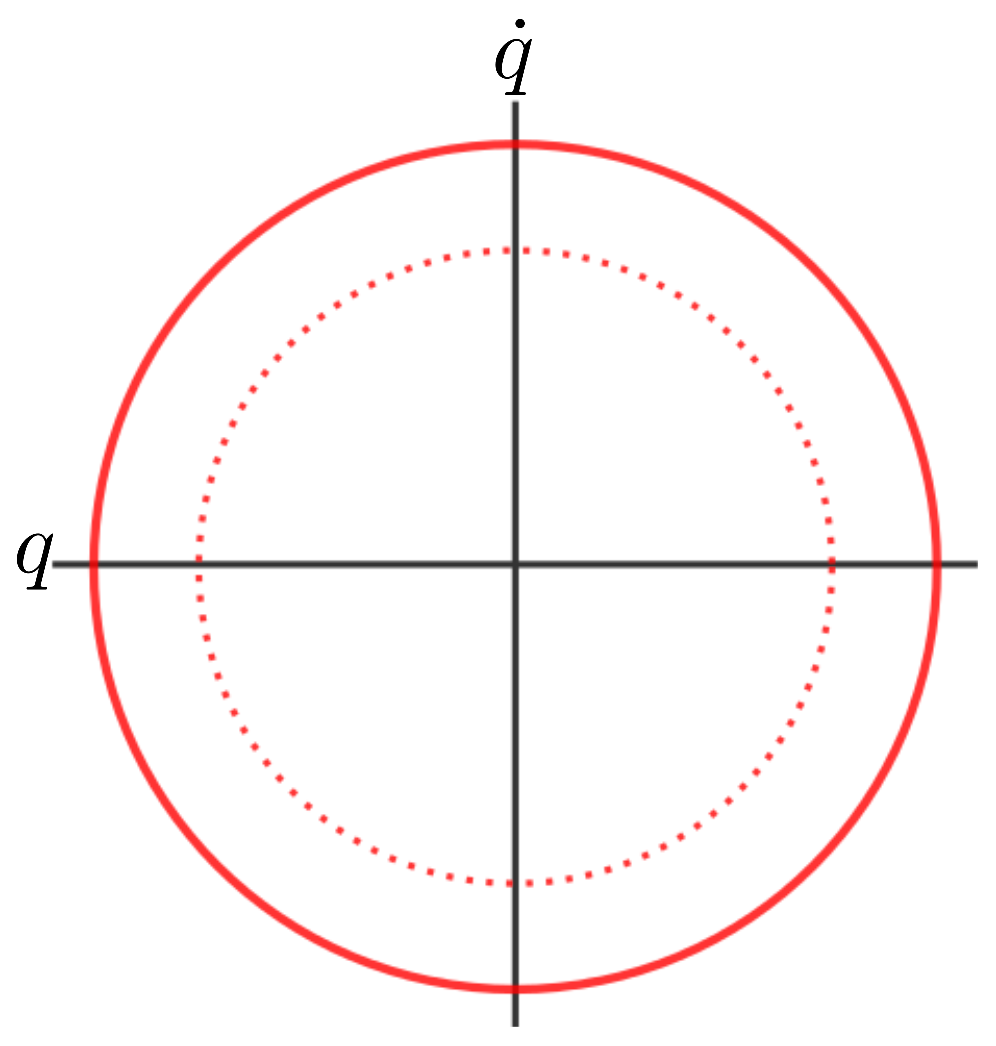
\includegraphics[width=0.7\textwidth]{g_en}
    \caption{Energe Scaling Action}
    \label{fig:gen}
\end{center}
\end{figure}


\subsection*{Time Offset}
we can also offset the time $t$
\[
t \mapsto t+\alpha
\]
\[
\gtd(\state(t))=[q(t+\alpha),\qd(t+\alpha)]
\]
For dynamic system, this seems obvious. And no control is need for such symmetry.
For system with limit circle, this $\gtd$ has a special effects like phase modification.

On phase plot, this has the effect rotate on the limit circle about an angle.
\begin{figure}[!htbp]
  \begin{center}
      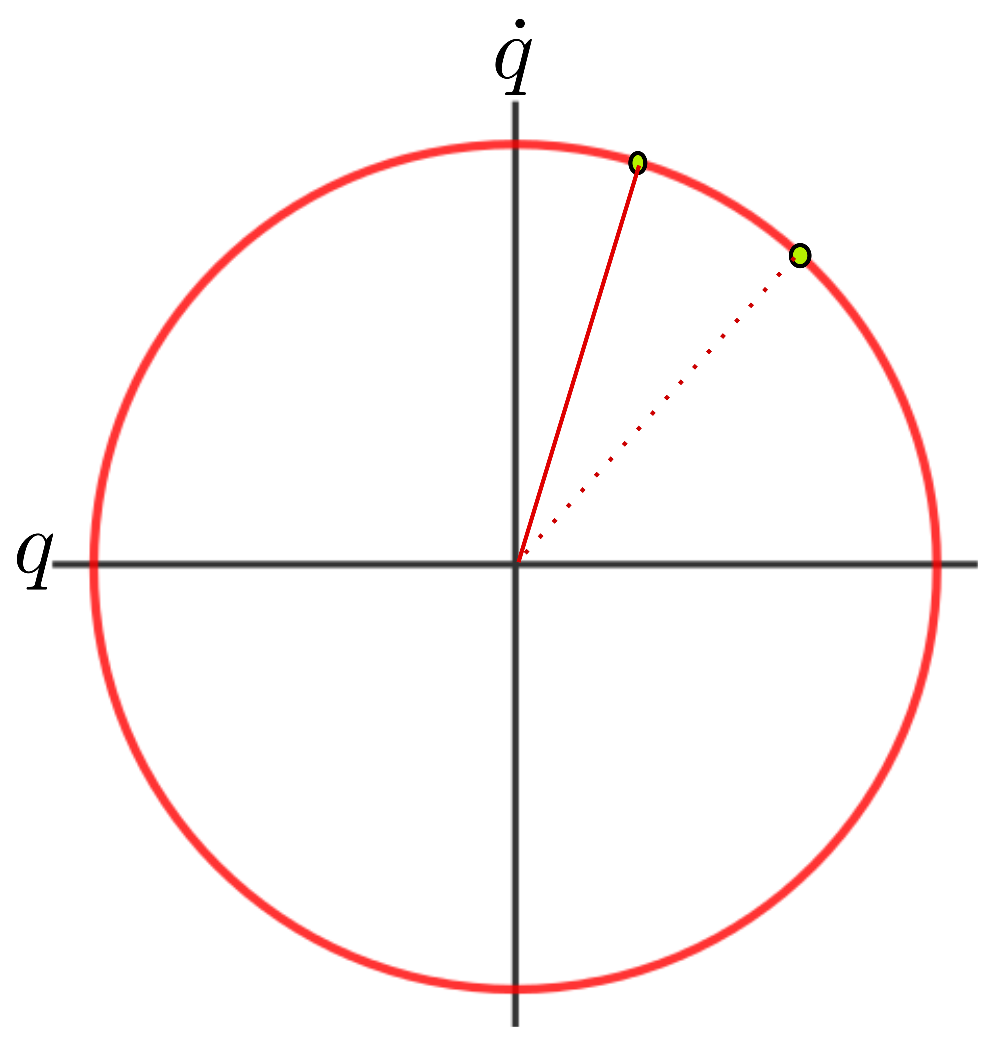
\includegraphics[width=0.7\textwidth]{g_toff}
    \caption{Offset Action}
    \label{fig:gtoff}
\end{center}
\end{figure}





\section{Example:Bouncing Ball dropt from Different Height}
Even it is a hybrid system,
The bouncing ball system has a energy scaling symmetry.

the energy function 
\[
E=g_{ravity}h+\frac{1}{2}m\qd^2
\]
so the 
\[
f(\alpha)=\alpha^2
\]

then the energy scaling action is
\[
\gen(\state)=[\alpha^2 q, \alpha \qd]
\]

given the motion of a ball dropt at 5 are shown in Figure~\ref{bouncing5}.


\begin{figure}[!htbp]
  \begin{center}
      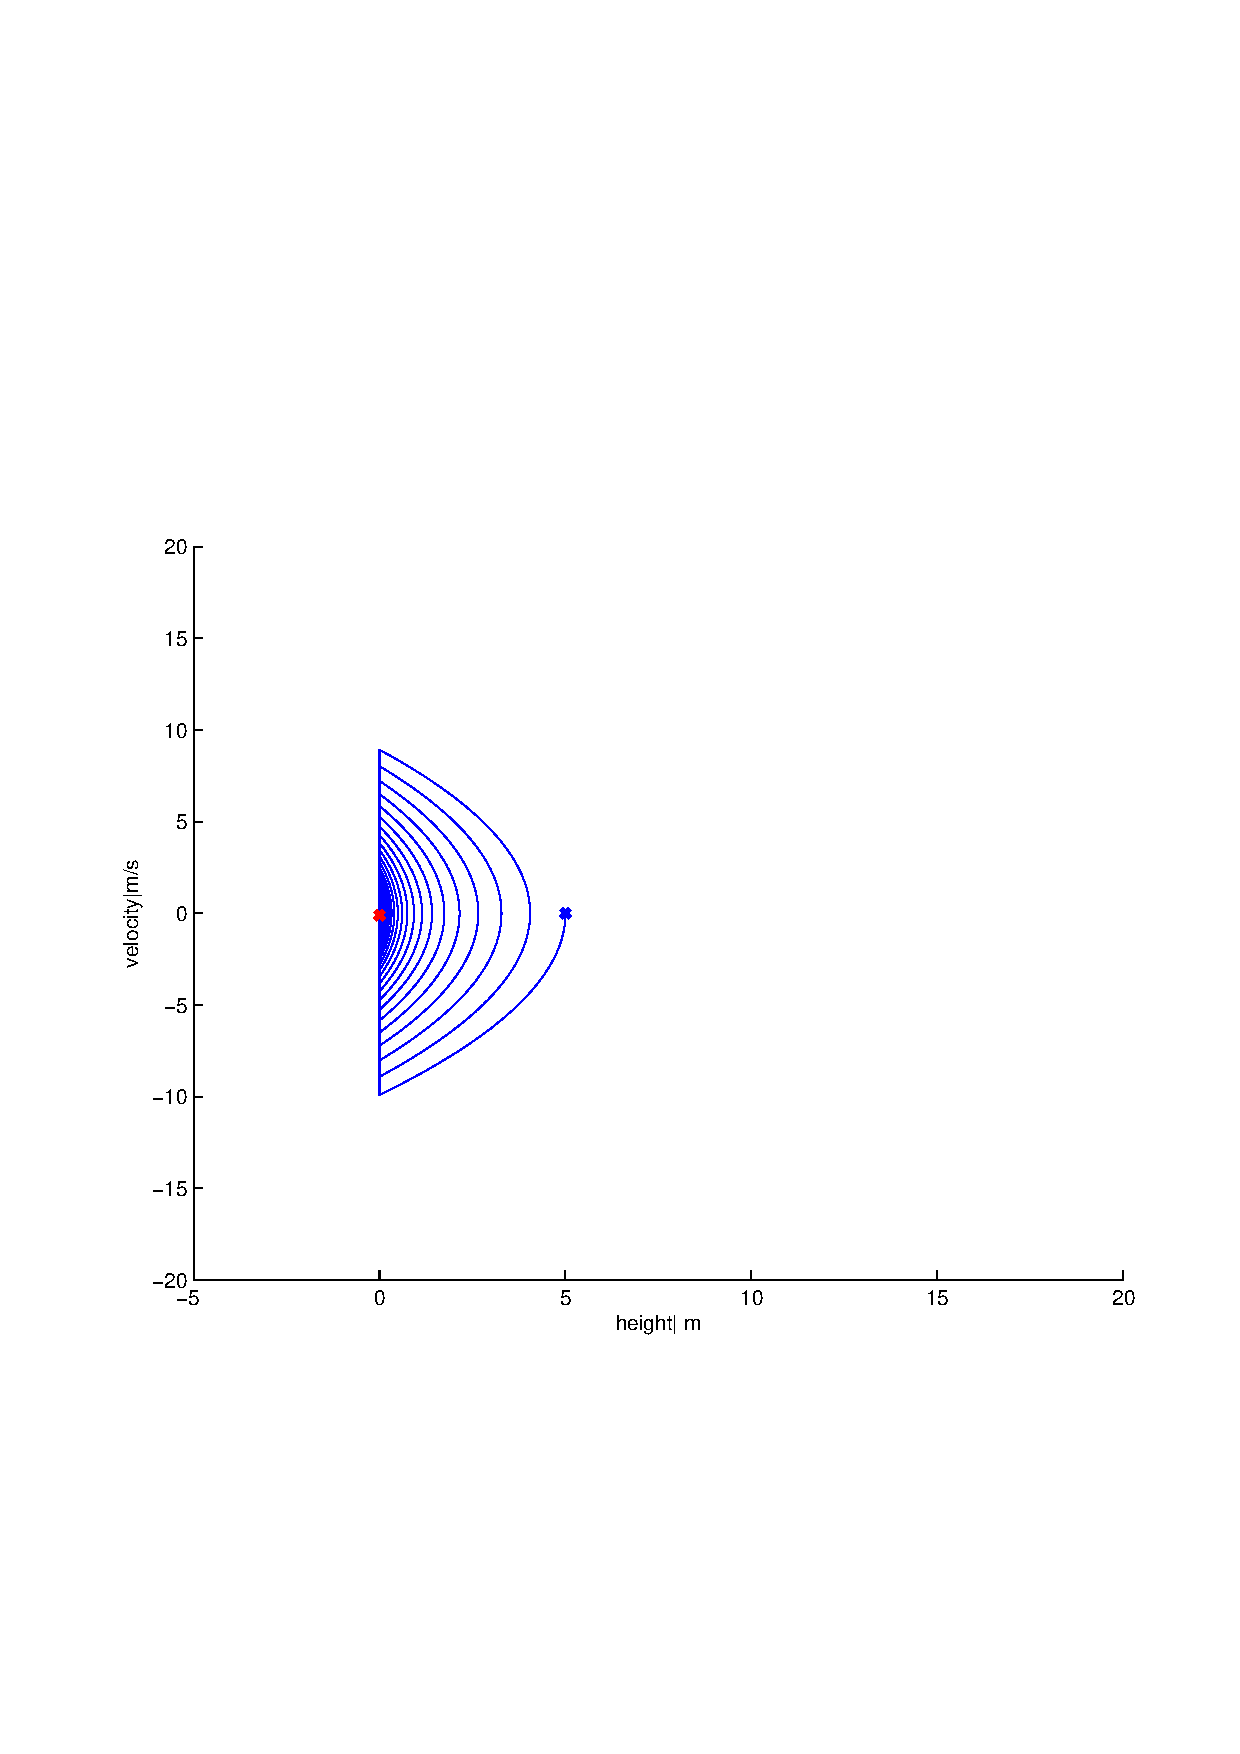
\includegraphics[width=0.7\textwidth]{BouncingBallPhasePlotuncontrolledDropAt5}
    \caption{Drop at 5}
    \label{fig:bouncing5}
\end{center}
\end{figure}

if $\alpha=\sqrt{2}$, we get the bouncing motion drop at height 10, as show in figure ~~\ref{bouncing5}
\begin{figure}[!htbp]
  \begin{center}
      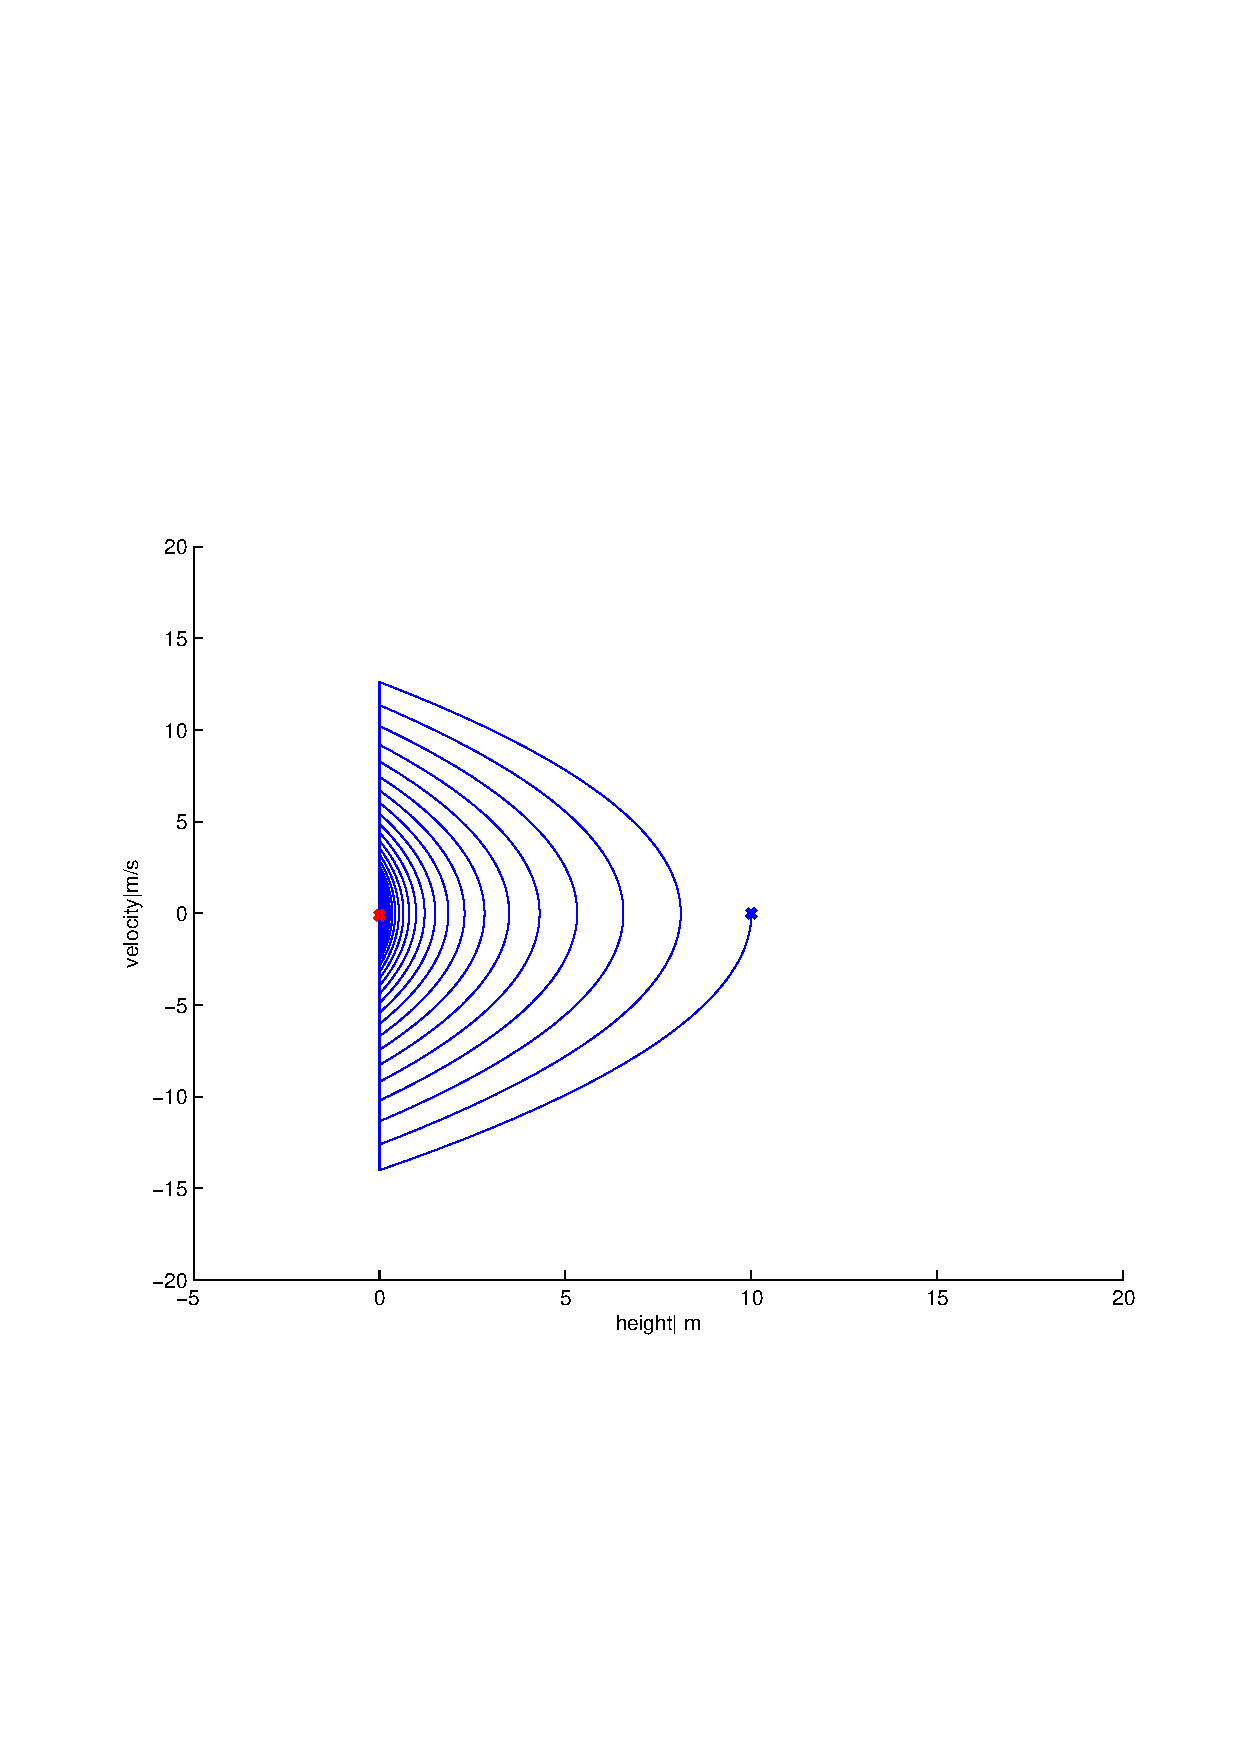
\includegraphics[width=0.7\textwidth]{BouncingBallPhasePlotuncontrolledDropAt10}
    \caption{Drop at 10}
    \label{fig:bouncing10}
\end{center}
\end{figure}


